\documentclass[12pt,a4paper]{article}
\usepackage{preamble}


\PassOptionsToPackage{
  backend=biber,
  style=numeric, % eller authoryear
  sorting=nyt,
  giveninits=true,
  maxbibnames=99,
  doi=false,isbn=false,url=true,
  dashed=false
}{biblatex}


\usepackage{preamble}
\usepackage{xcolor}
\usepackage{booktabs}
\usepackage{circuitikz}
\usepackage{float} % for [H] exact figure placement
\usetikzlibrary{arrows.meta}

\usepackage{pgfplots}
\pgfplotsset{compat=1.18}



\addbibresource{./referanser.bib}

% ------ Metadata ------
\newcommand{\institution}{Cyberingeniørskolen}
\newcommand{\coursecode}{ELE1000 Elektronikk}
\newcommand{\assignmenttype}{OBLIG 01}
\newcommand{\assignmenttitle}{DIODES IN CIRCUITS}
\newcommand{\assignmentno}{1}
\newcommand{\studentname}{Tor Johan Aleksandersen}
\newcommand{\class}{Elektronikk}
\newcommand{\submissiondate}{\today}

\begin{document}

% frontpage.tex
\thispagestyle{empty}

\begin{center}
    {\Large \bfseries \institution \\[1ex]}
    {\large \coursecode \\[6ex]}

    {\rule{0.9\textwidth}{1.5pt} \\[4ex]}

    {\fontsize{28}{32}\selectfont \bfseries \assignmenttype \\[3ex]}
    {\fontsize{20}{24}\selectfont \bfseries \assignmenttitle \\[2ex]}
    {\Large \bfseries Oppgave \assignmentno \\[6ex]}

    {\rule{0.9\textwidth}{1.5pt} \\[8ex]}

    {\large \bfseries Navn: \studentname \\[2ex]}
    {\large \bfseries Klasse: \class \\[2ex]}
    {\large \bfseries Dato: \submissiondate}
\end{center}

\vfill

\clearpage

\pagenumbering{arabic}
\setcounter{page}{1}

\section{Task 1}

\subsection{a)}

\begin{figure}[H]
\centering
\begin{circuitikz}[american voltages]

    % Nodes
    \node[circle, draw=black, fill=none, thick, inner sep=2pt] (V1) at (-3,0) {};
    \node[circle, fill=black, inner sep=0pt] (N1) at (-1,0) {};
    \node[circle, fill=black, inner sep=0pt] (N2) at (2,0) {};
    \node[circle, draw=black, fill=none, thick, inner sep=2pt] (V2) at (5,0) {};

    % Top and bottom branch nodes
    \node[circle, fill=black, inner sep=0pt] (T1) at (-1,1.5) {};
    \node[circle, fill=black, inner sep=0pt] (T2) at (2,1.5) {};
    \node[circle, fill=black, inner sep=0pt] (B1) at (-1,-1.5) {};
    \node[circle, fill=black, inner sep=0pt] (B2) at (2,-1.5) {};

    % Labels
    \node[left] at (V1) {+10V};
    \node[right] at (V2) {+6V};
    \node at (2.3,0.3) {$U_0$};

    % Left diode + current
    \draw (V1) to[short, -, i^=$I$] (-2,0)
          to[D, l_=Si] (N1);

    % Vertical connections (parallel network)
    \draw (N1) -- (T1);
    \draw (N1) -- (B1);
    \draw (N2) -- (T2);
    \draw (N2) -- (B2);

    % Parallel diodes
    \draw (T1) to[D, l=Ge] (T2);
    \draw (B1) to[D, l=Si] (B2);

    % Resistor to right source
    \draw (N2) to[R=$3\,\mathrm{k}\Omega$] (V2);

\end{circuitikz}
\caption{Diodekrets med parallelle grener og seriemotstand.}
\label{fig:diodekrets}
\end{figure}

\noindent
Since theres a definite enough voltage coming from the node on the left we can assume the first diode turns on and current goes. In the parallell branch we have two diodes, since the voltage difference over the parallell must equal, the $Ge$ diode must open first since it has lower threshold at $0.3V$ rather than $0.7$. The circuit change state to as shown under.

\begin{figure}[H]
\centering
\begin{circuitikz}[american voltages]

    % Nodes
    \node[circle, draw=black, fill=none, thick, inner sep=2pt] (V1) at (-3,0) {};
    \node[circle, fill=black, inner sep=0pt] (N1) at (-1,0) {};
    \node[circle, fill=black, inner sep=0pt] (N2) at (2,0) {};
    \node[circle, draw=black, fill=none, thick, inner sep=2pt] (V2) at (5,0) {};

    % Top and bottom branch nodes
    \node[circle, fill=black, inner sep=0pt] (T1) at (-1,1.5) {};
    \node[circle, fill=black, inner sep=0pt] (T2) at (2,1.5) {};
    \node[circle, fill=black, inner sep=0pt] (B1) at (-1,-1.5) {};
    \node[circle, fill=black, inner sep=0pt] (B2) at (2,-1.5) {};

    % Labels
    \node[left] at (V1) {+10V};
    \node[right] at (V2) {+6V};
    \node at (2.3,0.3) {$U_0$};

    % Left diode (0.7V drop)
    \draw (V1) to[short, -, i^=$I$] (-2,0)
          to[D, l_=0.7\,V] (N1);

    % Vertical connections
    \draw (N1) -- (T1);
    \draw (N2) -- (T2);

    % Top diode (Ge ON, 0.3V)
    \draw (T1) to[D, l=0.3\,V] (T2);

    % Bottom branch (open circuit)
    \draw (B1) -- ++(1,0) node[midway, below]{open};

    % Connect lower nodes visually (but not electrically through diode)
    \draw (N1) -- (B1);
    \draw (N2) -- (B2);

    % Resistor
    \draw (N2) to[R=$3\,\mathrm{k}\Omega$] (V2);

\end{circuitikz}
\caption{Diodekrets med aktiv Ge-diode og sperret Si-diode.}
\label{fig:diodekrets_aktiv}
\end{figure}



\noindent
\[
\begin{aligned}
    U_O &= 10V - 0.7V - 0.3V \\
    U_O &= 9V \\
    I &= \frac{3V}{3k\Omega} \\
    I &= 1.0mA
\end{aligned}
\]

\clearpage

\subsection{b)}

\begin{figure}[H]
\centering
\begin{circuitikz}[american voltages]

    % Nodes
    \node[circle, draw=black, fill=none, thick, inner sep=2pt] (V1) at (-4,0) {};
    \node[circle, fill=black, inner sep=0pt] (N1) at (-2,0) {};
    \node[circle, fill=black, inner sep=0pt] (T1) at (-2,1.5) {};
    \node[circle, fill=black, inner sep=0pt] (T2) at (0,1.5) {};
    \node[circle, fill=black, inner sep=0pt] (T3) at (2,1.5) {};
    \node[circle, fill=black, inner sep=0pt] (B1) at (-2,-1.5) {};
    \node[circle, fill=black, inner sep=0pt] (B2) at (0,-1.5) {};
    \node[circle, fill=black, inner sep=0pt] (N2) at (2,0) {};
    \node[circle, fill=black, inner sep=0pt] (N3) at (2,-1.5) {};
    \node[circle, draw=black, fill=none, thick, inner sep=2pt] (V2) at (3.5,0) {};

    % Labels
    \node[left] at (V1) {+10V};
    \node[right] at (V2) {$U_0$};

    % Left input wire
    \draw (V1) to[short] (N1);

    % Upper branch
    \draw (N1) -- (T1);
    \draw (T1) to[D, l_=Si] (T2);
    \draw (T2) to[R=$2\,\mathrm{k}\Omega$] (T3);

    % Lower branch
    \draw (N1) -- (B1);
    \draw (B1) to[D, l=Si] (B2);
    \draw (B2) to[R=$2\,\mathrm{k}\Omega$] (N3);

    % Right vertical connection
    \draw (N2) -- (V2);
    \draw (N2) -- (N3);
    \draw (T3) -- (N2);

    % Resistor to ground
    \draw (N3) to[R=$2\,\mathrm{k}\Omega$] (2,-3.2)
          node[ground]{};

    % Current arrow on top branch
    \draw[->] (-2, 2.2) -- (-1,2.2) node[midway, above] {$I$};

\end{circuitikz}
\caption{Diode circuit with two parallel branches and a load resistor to ground.}
\label{fig:diode_parallel_resistors}
\end{figure}

As the $+10V$ rises, $U_0$ stays at grounding ($0V$) since theres no current to change it through the resistor. The voltage drop over both branches are the same and the diodes will open at input voltage $0.7V$.
\clearpage

\section{Task 2}

\begin{figure}[H]
\centering
\begin{circuitikz}[american voltages]

    % Nodes
    \node[circle, draw=black, fill=none, thick, inner sep=2pt] (VinTop) at (-4,1.5) {};
    \node[circle, draw=black, fill=none, thick, inner sep=2pt] (VinBot) at (-4,-1.5) {};

    \node[circle, fill=black, inner sep=0pt] (N1) at (-0.3,1.5) {};
    \node[circle, fill=black, inner sep=0pt] (N2) at (-0.3,-1.5) {};
    \node[circle, fill=black, inner sep=0pt] (Top) at (1.5,1.5) {};
    \node[circle, fill=black, inner sep=0pt] (Bot) at (1.5,-1.5) {};

    \node[circle, draw=black, fill=none, thick, inner sep=2pt] (VoutTop) at (3.5,1.5) {};
    \node[circle, draw=black, fill=none, thick, inner sep=2pt] (VoutBot) at (3.5,-1.5) {};

    % Input voltage
    \draw (VinTop) to[open, v^=$U_i$] (VinBot);

    % Bottom rail
    \draw (VinBot) -- (Bot) -- (VoutBot);

    % Top path with resistor
    \draw (VinTop) to[R=$2\,\mathrm{k}\Omega$, i>^=$I_R$] (N1) -- (Top) -- (VoutTop);

    % Parallel branches
    \draw (N1) to[D, l=Si] (N2);                 % diode branch
    \draw (Top) to[R=$5\,\mathrm{k}\Omega$] (Bot); % resistor branch

    % Output voltage
    \draw (VoutTop) to[open, v^=$U_0$] (VoutBot);

\end{circuitikz}
\caption{Diode and resistor in parallel between output nodes.}
\label{fig:parallel_diode_resistor}
\end{figure}

\noindent
Before $U_0$ reach $0.7V$ all current pass through the $5k\Omega$ resistor. We then have this:
\[
I_R = \frac{U_i}{2k+5k} \quad U_0 = U_i - 2\left(\frac{U_i}{7k}\right)
\]

\noindent
By checking when $U_0$ equals 0.7 we solve for $U_i$ and get $U_i = 0.98V$. This means that when input voltage is greater than $0.98V$ we have output voltage of $0.7V$ constantly. When input is negative, the current is reversed and the diode shuts off, and in that case we can calculate output as.

\[
U_0 = 5k \cdot \left(\frac{U_i}{2k + 5k}\right) \rightarrow U_0 = U_i \cdot \frac{5}{7}
\]

\noindent
When the diode activates, the current will have a maximum of $9.3V$ going over the $2k$ resistor. When the diode is shut off, the current will be decided by voltage over resistor. The highest and lowest possible values are as below.

\[
I_{R\uparrow} = \frac{9.3V}{2k\Omega} = 4.65mA
\]
\[
U_{0\downarrow} = -10V \cdot \frac{5k\Omega}{2k\Omega + 5k\Omega} = -7.14V
\]
\[
I_{R\downarrow} = \frac{-7.14V}{5k\Omega} = -1.42mA
\]

\noindent
The graphs are shown below.

\begin{figure}[H]
\centering
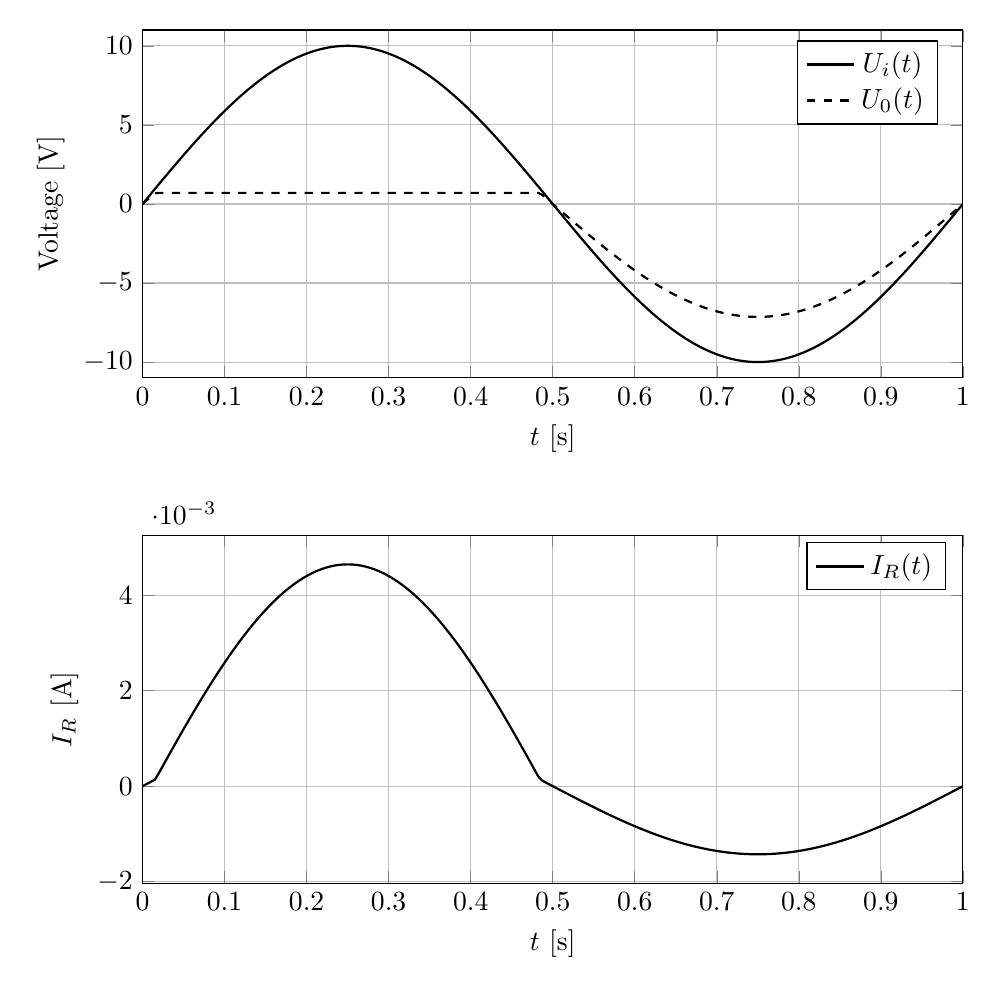
\begin{tikzpicture}

% ---- Voltage plot ----
\begin{axis}[
    width=12cm,
    height=6cm,
    xlabel={$t$ [s]},
    ylabel={Voltage [V]},
    xmin=0, xmax=1,
    ymin=-11, ymax=11,
    grid=both,
    legend pos=north east,
    domain=0:1,
    samples=200
]

\addplot[thick]
{10*sin(deg(2*pi*x))};
\addlegendentry{$U_i(t)$}

\addplot[thick, dashed]
{ (10*sin(deg(2*pi*x)) > 0.98) ? 0.7 : (5/7)*(10*sin(deg(2*pi*x))) };
\addlegendentry{$U_0(t)$}

\end{axis}

% ---- Current plot ----
\begin{axis}[
    at={(0,-2cm)},
    anchor=north west,
    width=12cm,
    height=6cm,
    xlabel={$t$ [s]},
    ylabel={$I_R$ [A]},
    xmin=0, xmax=1,
    grid=both,
    domain=0:1,
    samples=200
]

\addplot[thick]
{
(10*sin(deg(2*pi*x)) > 0.98)
? (10*sin(deg(2*pi*x)) - 0.7)/2000
: (10*sin(deg(2*pi*x)))/7000
};

\addlegendentry{$I_R(t)$}

\end{axis}

\end{tikzpicture}
\caption{Voltage and current in the diode circuit.}
\label{fig:diode_voltage_current}
\end{figure}
\clearpage

\section{Task 3}

\subsection{a)}

\begin{figure}[H]
\centering
\begin{circuitikz}[american voltages]

    % Bridge nodes
    \node[circle, fill=black, inner sep=0pt] (Top) at (0,2) {};
    \node[circle, fill=black, inner sep=0pt] (Right) at (2,0) {};
    \node[circle, fill=black, inner sep=0pt] (Bottom) at (0,-2) {};
    \node[circle, fill=black, inner sep=0pt] (Left) at (-2,0) {};

    % Source (input) inside bridge
    \draw (Top) to[open, v^=$U_i$] (Bottom);

    % Diodes (bridge)
    \draw (Top) to[D, l=$D_1$] (Right);
    \draw (Right) to[D, l=$D_2$] (Bottom);
    \draw (Bottom) to[D, l=$D_3$] (Left);
    \draw (Left) to[D, l=$D_4$] (Top);

    % Output resistor
    \node[circle, fill=black, inner sep=0pt] (OutTop1) at (4,0) {};
    \node[circle, fill=black, inner sep=0pt] (OutBot1) at (4,-3) {};
    \node[circle, fill=black, inner sep=0pt] (OutBot2) at (-2,-3) {};

    \draw (Right) -- (OutTop1);
    \draw (Left) -- (OutBot2);
    \draw (OutBot1) -- (OutBot2);

    \draw (OutTop1) to[R=$R$] (OutBot1);

    % Output voltage
    \draw (5, 0) to[open, l^=$U_0$] (5, -3);

    \node[ground] at (OutBot1) {};

    \draw[->, thick] (Top) -- (Right);
    \draw[->, thick] (Right) -- (OutTop1);
    \draw[->, thick] (OutBot1) -- (OutBot2);
    \draw[->, thick] (Left) -- (Bottom);
    \draw[->, thick] (Bottom) -- (Top);

\end{circuitikz}
\caption{Current direction in positive cycle}
\label{fig:bridge_rectifier}
\end{figure}

\begin{figure}[H]
\centering
\begin{circuitikz}[american voltages]

    % Bridge nodes
    \node[circle, fill=black, inner sep=0pt] (Top) at (0,2) {};
    \node[circle, fill=black, inner sep=0pt] (Right) at (2,0) {};
    \node[circle, fill=black, inner sep=0pt] (Bottom) at (0,-2) {};
    \node[circle, fill=black, inner sep=0pt] (Left) at (-2,0) {};

    % Source (input) inside bridge
    \draw (Top) to[open, v^=$U_i$] (Bottom);

    % Diodes (bridge)
    \draw (Top) to[D, l=$D_1$] (Right);
    \draw (Right) to[D, l=$D_2$] (Bottom);
    \draw (Bottom) to[D, l=$D_3$] (Left);
    \draw (Left) to[D, l=$D_4$] (Top);

    % Output resistor
    \node[circle, fill=black, inner sep=0pt] (OutTop1) at (4,0) {};
    \node[circle, fill=black, inner sep=0pt] (OutBot1) at (4,-3) {};
    \node[circle, fill=black, inner sep=0pt] (OutBot2) at (-2,-3) {};

    \draw (Right) -- (OutTop1);
    \draw (Left) -- (OutBot2);
    \draw (OutBot1) -- (OutBot2);

    \draw (OutTop1) to[R=$R$] (OutBot1);

    % Output voltage
    \draw (5, 0) to[open, l^=$U_0$] (5, -3);

    \node[ground] at (OutBot1) {};

    \draw[->, thick] (Bottom) -- (Right);
    \draw[->, thick] (Right) -- (OutTop1);
    \draw[->, thick] (OutBot1) -- (OutBot2);
    \draw[->, thick] (Left) -- (Top);
    \draw[->, thick] (Top) -- (Bottom);

\end{circuitikz}
\caption{Current direction in negative cycle}
\label{fig:bridge_rectifier}
\end{figure}


\noindent
Current in both cases flow in the same direction through the resistor, $R$. The diodes are ideal and there is no voltage drop over any component, except for the resistor. So the fall of potential over the resistor must equal the total input voltage. We can graph it as shown below.

\begin{figure}[H]
\centering
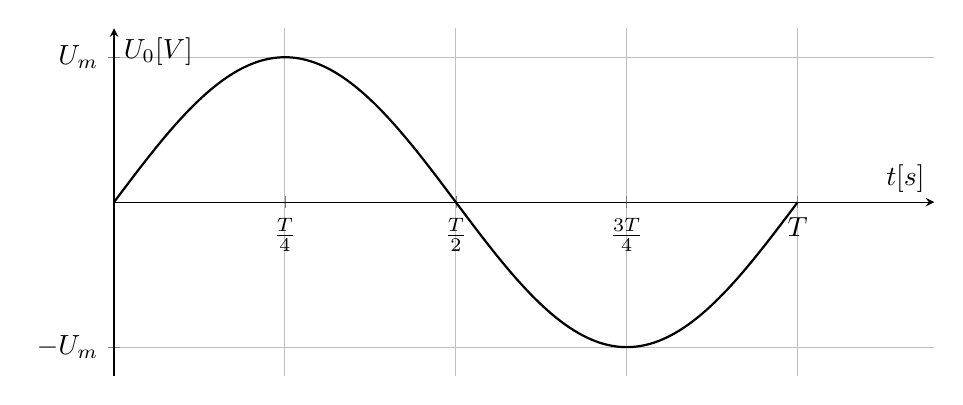
\begin{tikzpicture}
\begin{axis}[
    width=12cm,
    height=6cm,
    xlabel={$t [s]$},
    ylabel={$U_0 [V]$},
    xmin=0, xmax=1.2,
    ymin=-1.2, ymax=1.2,
    axis lines=middle,
    xtick={0,0.25,0.5,0.75,1},
    xticklabels={$0$, $\frac{T}{4}$, $\frac{T}{2}$, $\frac{3T}{4}$, $T$},
    ytick={-1,1},
    yticklabels={$-U_m$, $U_m$},
    grid=both,
    domain=0:1,
    samples=200
]

\addplot[thick]
{sin(deg(2*pi*x))};

\end{axis}
\end{tikzpicture}
\caption{Voltage over resistor.}
\end{figure}

\subsection{b)}

\begin{figure}[H]
\centering
\begin{circuitikz}[american voltages]

    % Bridge nodes
    \node[circle, fill=black, inner sep=0pt] (Top) at (0,2) {};
    \node[circle, fill=black, inner sep=0pt] (Right) at (2,0) {};
    \node[circle, fill=black, inner sep=0pt] (Bottom) at (0,-2) {};
    \node[circle, fill=black, inner sep=0pt] (Left) at (-2,0) {};

    % Source (input) inside bridge
    \draw (Top) to[open, v^=$U_i$] (Bottom);

    % Diodes (bridge)
    \draw (Top) to[D, l=$D_1$] (Left);
    \draw (Bottom) to[D, l=$D_3$] (Left);
    \draw (Right) to[D, l=$D_2$] (Top);
    \draw (Right) to[D, l=$D_4$] (Bottom);

    % Output resistor
    \node[circle, fill=black, inner sep=0pt] (OutTop1) at (4,0) {};
    \node[circle, fill=black, inner sep=0pt] (OutBot1) at (4,-3) {};
    \node[circle, fill=black, inner sep=0pt] (OutBot2) at (-2,-3) {};

    \draw (Right) -- (OutTop1);
    \draw (Left) -- (OutBot2);
    \draw (OutBot1) -- (OutBot2);

    \draw (OutTop1) to[R=$R$] (OutBot1);

    % Output voltage
    \draw (5, 0) to[open, l^=$U_0$] (5, -3);

    \node[ground] at (OutBot1) {};

    \draw[->, thick] (Top) -- (Left);
    \draw[->, thick] (OutTop1) -- (Right);
    \draw[->, thick] (OutBot2) -- (OutBot1);
    \draw[->, thick] (Right) -- (Bottom);
    \draw[->, thick] (Bottom) -- (Top);

\end{circuitikz}
\caption{Current direction in positive cycle}
\label{fig:bridge_rectifier}
\end{figure}


\begin{figure}[H]
\centering
\begin{circuitikz}[american voltages]

    % Bridge nodes
    \node[circle, fill=black, inner sep=0pt] (Top) at (0,2) {};
    \node[circle, fill=black, inner sep=0pt] (Right) at (2,0) {};
    \node[circle, fill=black, inner sep=0pt] (Bottom) at (0,-2) {};
    \node[circle, fill=black, inner sep=0pt] (Left) at (-2,0) {};

    % Source (input) inside bridge
    \draw (Top) to[open, v^=$U_i$] (Bottom);

    % Diodes (bridge)
    \draw (Top) to[D, l=$D_1$] (Left);
    \draw (Bottom) to[D, l=$D_3$] (Left);
    \draw (Right) to[D, l=$D_2$] (Top);
    \draw (Right) to[D, l=$D_4$] (Bottom);

    % Output resistor
    \node[circle, fill=black, inner sep=0pt] (OutTop1) at (4,0) {};
    \node[circle, fill=black, inner sep=0pt] (OutBot1) at (4,-3) {};
    \node[circle, fill=black, inner sep=0pt] (OutBot2) at (-2,-3) {};

    \draw (Right) -- (OutTop1);
    \draw (Left) -- (OutBot2);
    \draw (OutBot1) -- (OutBot2);

    \draw (OutTop1) to[R=$R$] (OutBot1);

    % Output voltage
    \draw (5, 0) to[open, l^=$U_0$] (5, -3);

    \node[ground] at (OutBot1) {};

    \draw[->, thick] (Bottom) -- (Left);
    \draw[->, thick] (OutTop1) -- (Right);
    \draw[->, thick] (OutBot2) -- (OutBot1);
    \draw[->, thick] (Right) -- (Top);
    \draw[->, thick] (Top) -- (Bottom);

\end{circuitikz}
\caption{Current direction in negative cycle}
\label{fig:bridge_rectifier}
\end{figure}

\noindent
The only drop of voltage is over the resistor, but now the current is reversed. So the graph is the negative of the input.

\begin{figure}[H]
\centering
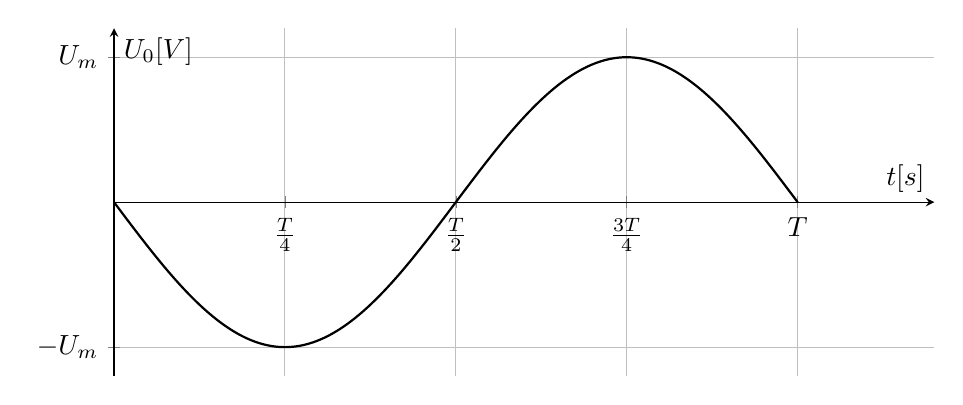
\begin{tikzpicture}
\begin{axis}[
    width=12cm,
    height=6cm,
    xlabel={$t [s]$},
    ylabel={$U_0 [V]$},
    xmin=0, xmax=1.2,
    ymin=-1.2, ymax=1.2,
    axis lines=middle,
    xtick={0,0.25,0.5,0.75,1},
    xticklabels={$0$, $\frac{T}{4}$, $\frac{T}{2}$, $\frac{3T}{4}$, $T$},
    ytick={-1,1},
    yticklabels={$-U_m$, $U_m$},
    grid=both,
    domain=0:1,
    samples=200
]

\addplot[thick]
{-sin(deg(2*pi*x))};

\end{axis}
\end{tikzpicture}
\caption{Voltage over resistor.}
\end{figure}
\clearpage

\section{Task 4}

\begin{figure}[H]
\centering
\begin{circuitikz}[american voltages]

    % Nodes
    \node[circle, draw=black, fill=none, thick, inner sep=2pt] (Vtop) at (-3,1.5) {};
    \node[circle, draw=black, fill=none, thick, inner sep=2pt] (Vbot) at (-3,-1.5) {};

    \node[circle, fill=black, inner sep=0pt] (N1) at (-1,1.5) {};
    \node[circle, fill=black, inner sep=0pt] (N2) at (2,1.5) {};
    \node[circle, fill=black, inner sep=0pt] (N3) at (2,-1.5) {};
    

    % Voltage source
    \draw (Vtop) to[V=$20\,\mathrm{V}$] (Vbot);

    % Bottom rail
    \draw (Vbot) -- (N3);

    % Series resistor
    \draw (Vtop) -- (N1)
          to[R=$R_S$] (N2);

    % Top wire to load
    \draw (N2) -- ++(2,0) coordinate (TopR);
    \draw (N3) -- ++(2,0) coordinate (TopB);

    % Zener diode branch
    \draw (N3) to[zzD, l=$Z$] (N2);

    % Load resistor
    \draw (TopR) to[R=$R_L$] (TopB);

\end{circuitikz}
\caption{Zener diode voltage regulator circuit.}
\label{fig:zener_regulator}
\end{figure}

\noindent
With the given values.
\[
R_S = 220\Omega \quad U_Z = 10V \quad P_{Zmax} = 430mW
\]

\subsection{a. $R_L = 180\Omega$}

\[
\begin{aligned}
    U_{RL} &= 20 \cdot \frac{R_L}{R_S + R_L} = 9V, \quad \text{zenor diode stays open} \\
    I_{RL} &= \frac{9V}{180\Omega} = 50mA \\
    I_Z &= 0A \quad I_{RS} = I_{RL} = 50mA
\end{aligned}
\]

\subsection{b. $R_L = 470\Omega$}
\[
\begin{aligned}
    U_{RL} &= 20 \cdot \frac{R_L}{R_S + R_L} = 13.62V, \quad \text{zenor diode turns on} \\
    U_{RL} &= U_Z = 10V \\
    I_{RL} &= \frac{10V}{470\Omega} = 21mA \\
    I_{RS} &= \frac{20V - 10V}{220\Omega} = 45mA \\
    I_Z &= 45mA - 21mA = 24mA
\end{aligned}
\]

\subsection{c. $R_L$ at max zenor power}
\[
\begin{aligned}
    P_{Z\uparrow} &= V_Z \cdot I_Z \\
    430mW &= 10V \cdot I_Z \\
    I_Z &= 43mA \\
    I_{RS} &= 45mA \\
    R_L &= \frac{10V}{45mA - 43mA} = 5k\Omega
\end{aligned}
\]

\subsection{d. smallest value for $R_L$}
We can clearly see that input voltage is double the zenor voltage, in a perfect resistor dividing network. That means that the load resistanse must equal the input resistance. We can also calculate it as below.
\[
R_{L\downarrow} = \frac{V_Z R_S}{V_i - V_Z} = 220\Omega
\]
\clearpage

\section{Task 5}


\begin{figure}[H]
\centering
\begin{circuitikz}[american voltages]

    % Nodes
    \node[circle, draw=black, fill=none, thick, inner sep=2pt] (Vtop) at (-3,1.5) {};
    \node[circle, draw=black, fill=none, thick, inner sep=2pt] (Vbot) at (-3,-1.5) {};

    \node[circle, fill=black, inner sep=0pt] (N1) at (-1,1.5) {};
    \node[circle, fill=black, inner sep=0pt] (N2) at (2,1.5) {};
    \node[circle, fill=black, inner sep=0pt] (N3) at (2,-1.5) {};
    

    % Voltage source
    \draw (Vtop) to[vsourcesin, l=$10\sin(2\pi 50 t)$] (Vbot);

    % Bottom rail
    \draw (Vbot) -- (N3);

    % Series resistor
    \draw (Vtop) -- (N1)
          to[R=$R_1$] (N2);

    % Top wire to load
    \draw (N2) -- ++(3,0) coordinate (TopR);
    \draw (N3) -- ++(3,0) coordinate (TopB);

    \draw (TopR) -- ++(3,0) coordinate (Vt);
    \draw (TopB) -- ++(3,0) coordinate (Vb);

    \draw (Vt) to[open, v=$U_0$] (Vb);

    % Zener diode branch
    \draw (N3) to[zzD, l=$Z_1$, a=$6.8V$] (N2);

    % Load resistor
    \draw (TopR) to[zzD, a=$Z_2$, l=$3.9V$] (TopB);

\end{circuitikz}
\caption{}
\end{figure}

\noindent
Since we have diodes in both directions of a parallell, and they both have zenor voltages higher than $0.7V$. Regarding current direction and voltage, one zenor will open and the other turn on. That means that maximum voltage potential difference over the parallell branch is $\pm 0.7V$. We can graph $U_0(t)$ and $U_i(t)$.

\begin{figure}[H]
\centering
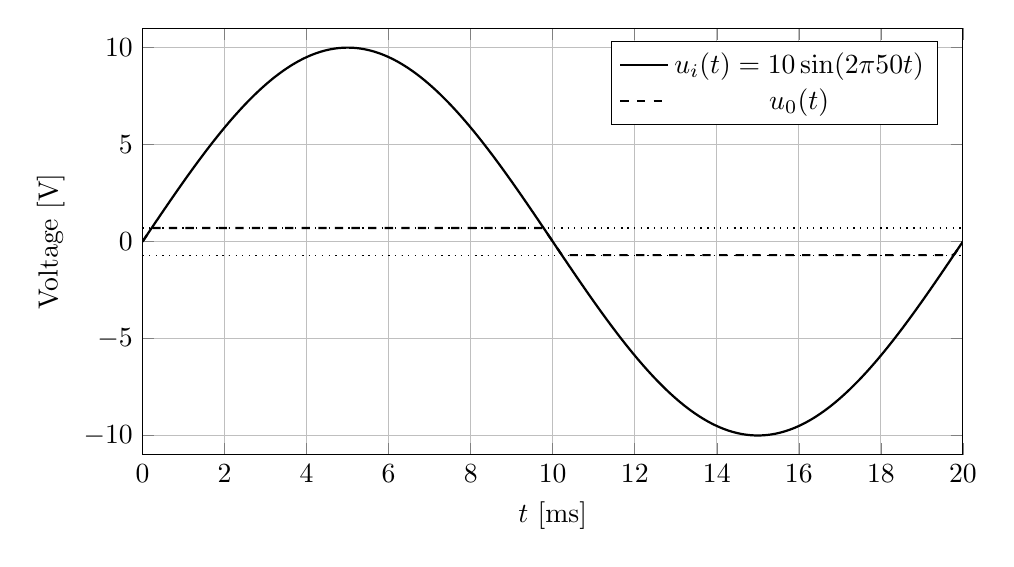
\begin{tikzpicture}
\begin{axis}[
    width=12cm,
    height=7cm,
    xlabel={$t$ [ms]},
    ylabel={Voltage [V]},
    xmin=0, xmax=20,
    ymin=-11, ymax=11,
    grid=both,
    legend pos=north east,
    domain=0:20,
    samples=400
]

% Input
\addplot[thick]
{10*sin(deg(2*pi*50*x/1000))};
\addlegendentry{$u_i(t)=10\sin(2\pi 50t)$}

% Output
\addplot[thick, dashed]
{
(10*sin(deg(2*pi*50*x/1000)) > 0.7) * 0.7
+
(10*sin(deg(2*pi*50*x/1000)) < -0.7) * (-0.7)
+
and(10*sin(deg(2*pi*50*x/1000)) >= -0.7, 10*sin(deg(2*pi*50*x/1000)) <= 0.7)
* (10*sin(deg(2*pi*50*x/1000)))
};
\addlegendentry{$u_0(t)$}

% Reference lines
\addplot[dotted] {0.7};
\addplot[dotted] {-0.7};

\end{axis}
\end{tikzpicture}
\caption{Input and clipped output voltage.}
\label{fig:zener_clipping}
\end{figure}

\noindent
The circuit will have no flowing current whenever the diodes are open circuit. When $| U_0(t) | > 0.7V$, there will be current flowing. The absolute max current is as below.

\[
I_{tot\uparrow} = \frac{10V - 0.7V}{1k\Omega} = 9.3mA
\]

\noindent
The graph of the current is as shown under.

\begin{figure}[H]
\centering
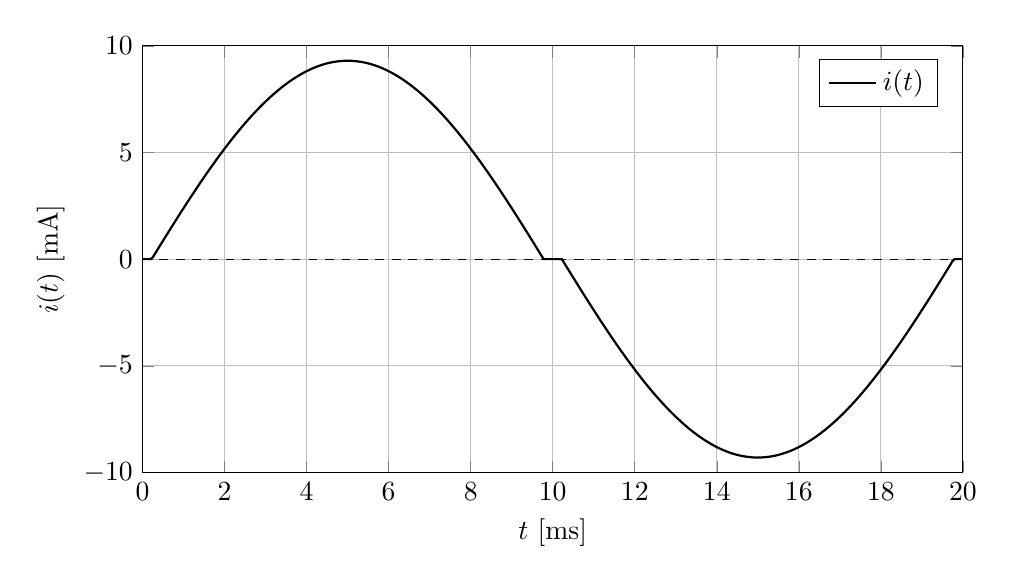
\begin{tikzpicture}
\begin{axis}[
    width=12cm,
    height=7cm,
    xlabel={$t$ [ms]},
    ylabel={$i(t)$ [mA]},
    xmin=0, xmax=20,
    ymin=-10, ymax=10,
    grid=both,
    legend pos=north east,
    domain=0:20,
    samples=400
]

% Current (mA)
\addplot[thick]
{
1000 * (
(10*sin(deg(2*pi*50*x/1000)) > 0.7)
* ((10*sin(deg(2*pi*50*x/1000)) - 0.7)/1000)
+
(10*sin(deg(2*pi*50*x/1000)) < -0.7)
* ((10*sin(deg(2*pi*50*x/1000)) + 0.7)/1000)
)
};
\addlegendentry{$i(t)$}

% Zero line
\addplot[dashed] {0};

\end{axis}
\end{tikzpicture}
\caption{Current with diode threshold.}
\label{fig:current_plot_signed}
\end{figure}
\clearpage

\printbibliography[heading=bibintoc,title={Referanser}]
\clearpage


%\section*{Vedlegg}
%\addcontentsline{toc}{section}{Vedlegg}
%\input{sections/vedlegg}
%\clearpage

\end{document}
